\documentclass[10pt,conference]{IEEEtran}

\usepackage{booktabs}
\usepackage{newtxtext}
\usepackage{newtxmath}
\usepackage{microtype}
\usepackage{tabularx}
\usepackage{xcolor}
\usepackage{hyperref}
\usepackage{tikz}
\usepackage{pgfplots}
\usepackage{flushend}
\usepackage{cite}

\usetikzlibrary{arrows.meta,positioning,fit,calc,shapes.geometric}
\pgfplotsset{compat=1.18}

\definecolor{huntrixblue}{HTML}{1F5A7A}
\definecolor{huntrixteal}{HTML}{2A8C82}
\definecolor{huntrixgold}{HTML}{D59B32}
\definecolor{huntrixred}{HTML}{B5483A}
\definecolor{huntrixgray}{HTML}{EEF2F4}

\hypersetup{
  colorlinks=true,
  linkcolor=huntrixblue,
  citecolor=huntrixblue,
  urlcolor=huntrixblue,
  pdftitle={Evidence-First Bengali Hallucination Detection},
  pdfauthor={Touhidul Alam Seyam, MD. Abtahee Kabir, Joyeta Barua Moni, and Noore Tamanna Orny},
  pdfsubject={Technical report for the IUT 12th ICT FEST Datathon},
  pdfkeywords={Bengali, hallucination detection, selective inference, evidence routing, Kaggle}
}

\newcommand{\labelzero}{\texttt{label=0}}
\newcommand{\labelone}{\texttt{label=1}}
\newcommand{\code}[1]{\texttt{\small #1}}

\begin{document}

\title{Evidence-First Bengali Hallucination Detection:\\
A Deterministic Selective Cascade}

\author{
\IEEEauthorblockN{
Touhidul Alam Seyam\IEEEauthorrefmark{1},
MD. Abtahee Kabir\IEEEauthorrefmark{2},
Joyeta Barua Moni\IEEEauthorrefmark{2},
Noore Tamanna Orny\IEEEauthorrefmark{2}
}
\IEEEauthorblockA{
\IEEEauthorrefmark{1}BGC Trust University Bangladesh\\
\IEEEauthorrefmark{2}Chittagong University of Engineering \& Technology\\
Team Huntrix, IUT 12th ICT FEST Datathon, July 2026\\
\href{https://github.com/Seyamalam/bengali-hallucination-v91-submission}{Public reproducibility package}}
}

\maketitle

\begin{abstract}
Our Bengali hallucination detector treats the benchmark as a mixture of tasks rather than one binary prompt. Source-lineage checks, structured solvers, context grounding, lexical and legal evidence, and relation-typed fact records decide high-confidence cases. A quantized open-weight model sees only the unresolved rows. Public macro-F1 rose from 0.657 to 0.967; the final Phase 1 result was private macro-F1 0.982 and rank 1. On the 299 released labels, the full cascade obtains 0.9933 macro-F1, while deterministic stages cover 225 rows without error. Three offline Kaggle runs on two Tesla T4 GPUs reproduced the scored 2,516-row CSV byte for byte in 440.87 to 593.43 seconds. A 5,000-row same-mix test took 14.60 minutes. Even an all-uncertain estimate stays below the nine-hour limit. The notebook computes every prediction from raw rows and pinned public assets; it does not load a saved prediction vector.
\end{abstract}

\begin{IEEEkeywords}
Bengali, hallucination detection, selective inference, evidence routing, reproducibility
\end{IEEEkeywords}

\section{Task and Design}

Each competition row contains an optional Bengali context, a prompt, and a model response. A fabricated, unsupported, or factually wrong response receives \labelzero; a faithful response receives \labelone. The released development set contains 299 labeled rows, whereas Phase 1 contains 2,516 unlabeled rows and Phase 2 is expected to contain about 5,000 rows from broader sources \cite{competition,phase2}.

The rows do not form one uniform classification task. They include context entailment, arithmetic, multiple-choice questions, Bengali morphology, idioms, legislation, historical dates, literature, and civic information. A single prompt forces one model to solve all of these relations with the same evidence policy. Early experiments showed that this was accurate enough to establish a baseline but unstable across the released set and the public leaderboard.

We changed the decision rule to \emph{selective resolution}. A rule or evidence source may emit a label only when its scope and relation are explicit. Everything else is deferred to a bounded LLM judge. The design has three practical goals:

\begin{enumerate}
  \item preserve high recall for hallucinated responses, the \labelzero\ class;
  \item avoid treating semantically related retrieval as ground truth;
  \item reproduce the same CSV offline on Kaggle T4$\times$2 within nine hours.
\end{enumerate}

The resulting system couples a trust-aware deterministic router with a small, fixed inference tail. The router reduces the cost and variance of LLM judging; the judge handles cases that do not fit a defensible exact rule.

\section{System}

\begin{figure*}[t]
\centering
\resizebox{0.96\textwidth}{!}{%
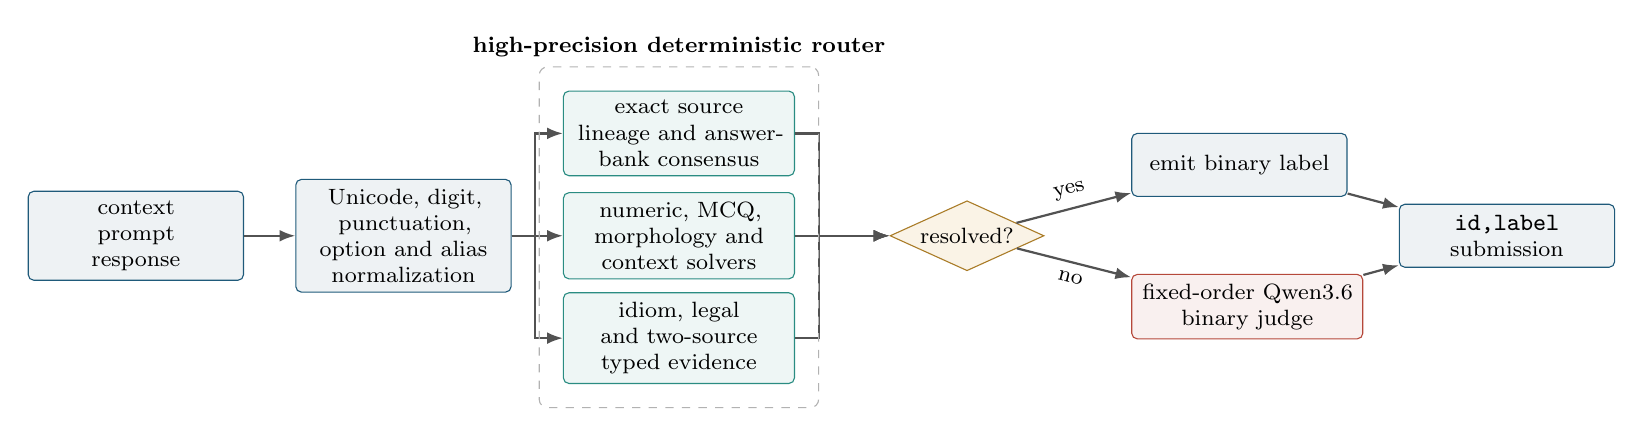
\begin{tikzpicture}[
  node distance=5.5mm and 6.5mm,
  every node/.style={font=\footnotesize},
  stage/.style={draw=huntrixblue, rounded corners=2pt, fill=huntrixgray,
                minimum height=8mm, align=center, text width=25mm},
  evidence/.style={draw=huntrixteal, rounded corners=2pt, fill=huntrixteal!8,
                   minimum height=8mm, align=center, text width=27mm},
  decision/.style={diamond, draw=huntrixgold!80!black, fill=huntrixgold!12,
                   aspect=2.2, align=center, inner sep=1.5pt},
  judge/.style={draw=huntrixred, rounded corners=2pt, fill=huntrixred!8,
                minimum height=8mm, align=center, text width=27mm},
  arrow/.style={-{Latex[length=2mm]}, thick, draw=black!68}
]
\node[stage] (input) {context\\prompt\\response};
\node[stage, right=of input] (norm) {Unicode, digit, punctuation, option and alias normalization};
\node[evidence, right=of norm, yshift=13mm] (lineage) {exact source lineage and answer-bank consensus};
\node[evidence, right=of norm] (structured) {numeric, MCQ, morphology and context solvers};
\node[evidence, right=of norm, yshift=-13mm] (typed) {idiom, legal and two-source typed evidence};
\node[decision, right=12mm of structured] (resolved) {resolved?};
\node[stage, right=11mm of resolved, yshift=9mm] (emit) {emit binary label};
\node[judge, right=11mm of resolved, yshift=-9mm] (llm) {fixed-order Qwen3.6\\binary judge};
\node[stage, right=of emit, yshift=-9mm] (csv) {\code{id,label}\\submission};

\draw[arrow] (input) -- (norm);
\draw[arrow] (norm.east) -- ++(3mm,0) |- (lineage.west);
\draw[arrow] (norm) -- (structured);
\draw[arrow] (norm.east) -- ++(3mm,0) |- (typed.west);
\draw[arrow] (lineage.east) -- ++(3mm,0) |- (resolved.west);
\draw[arrow] (structured) -- (resolved);
\draw[arrow] (typed.east) -- ++(3mm,0) |- (resolved.west);
\draw[arrow] (resolved) -- node[above,sloped]{yes} (emit);
\draw[arrow] (resolved) -- node[below,sloped]{no} (llm);
\draw[arrow] (emit) -- (csv);
\draw[arrow] (llm) -- (csv);

\node[draw=black!30, dashed, rounded corners=3pt, fit=(lineage)(structured)(typed),
      label={[font=\footnotesize\bfseries]above:high-precision deterministic router},
      inner sep=3mm] {};
\end{tikzpicture}
}
\caption{Frozen v91 inference path. Deterministic stages label only relation-matched cases. The open-weight judge receives the unresolved tail, not the full test set.}
\label{fig:architecture}
\end{figure*}

\subsection{Normalization and Task Routing}

The first stage normalizes Bengali and Latin digits, Unicode punctuation, spacing, answer aliases, and inline options. It also identifies whether context is absent, evidential, or merely instructional. This distinction matters: in several grammar examples the context describes the task rather than supplying the answer.

Exact lineage checks recover released BenHallu-style records and public question-answer sources only when normalized prompt, response, and relevant context fields agree. Reliability-weighted answer banks may resolve a row when their accepted answer relation is unambiguous. Approximate matches can propose a candidate, but they cannot overrule an exact source or an intrinsic context contradiction.

\subsection{Structured Solvers}

Small deterministic solvers handle arithmetic, numeric ranges, Bengali compound number words, multiple-choice serialization, morphology, compounds, and prefixes. Relation guards bind a date or number to the clause containing the requested entity and predicate. This prevents a valid year in the same passage from answering the wrong birth, death, publication, or establishment question.

For context rows, the system compares response claims with the supplied passage. Exact answer spans are accepted only inside a semicolon-aware clause that also contains prompt anchors. Named entities, dates, negation, and alternatives are checked before any external fact can contribute. The supplied context takes precedence over outside plausibility.

\subsection{Evidence Hierarchy}

Table~\ref{tab:evidence} summarizes the admission policy. An authoritative exact lineage source can decide alone. Conflicting answer banks require weighted agreement. Free-form factual records require at least two independent public sources and an explicit relation type. Idiom records distinguish the figurative meaning requested by the prompt from a literal gloss. These restrictions were added after broader retrieval produced plausible but incorrectly related evidence.

\begin{table}[t]
\caption{Evidence admission policy}
\label{tab:evidence}
\centering
\footnotesize
\begin{tabularx}{\columnwidth}{@{}p{0.27\columnwidth}X@{}}
\toprule
Evidence family & Condition required to emit a label \\
\midrule
Exact lineage & Prompt, response, and applicable context agree \\
Answer banks & Relation match and reliability-weighted consensus \\
Structured rule & Parsed operands, entity, and predicate all align \\
Context evidence & Same clause plus prompt anchors; no contradiction \\
Idiom or law & Exact headword/section and requested sense or provision \\
Free-form fact & Typed relation and two independent recorded sources \\
Fuzzy retrieval & Candidate generation only; never a stronger override \\
\bottomrule
\end{tabularx}
\end{table}

\subsection{Conflict Resolution and Abstention}

The router records a source family, relation, and confidence with each proposed decision. Intrinsic context contradiction has the highest priority because the task asks whether the answer follows the supplied passage. An exact authoritative source comes next, followed by relation-aligned structured parsing and consensus evidence. Fuzzy retrieval never decides a row by itself.

Conflicting proposals are not averaged blindly. If two sources claim different relations, both are discarded for that question. If they claim the same relation but disagree on the answer, the system requires a stronger exact source or abstains. This policy increased the judge queue in a few places, but it prevented weak retrieval from flipping labels that a trusted source had already resolved.

\subsection{Selective Open-Weight Judge}

After routing, 158 Phase 1 rows remain unresolved. They are sorted by row ID and processed in fixed batches. Context rows receive one context-NLI view. No-context rows receive up to three short views: factual verification, strict exam grading, and a zero-bias check. A faithful decision requires unanimous positive votes; evaluation stops after the first zero.

The judge uses Qwen3.6-27B Q4\_K\_P, a 16.332~GiB GGUF checkpoint, served by pinned \texttt{llama.cpp} b9637 across two T4 GPUs \cite{qwen,llamacpp}. Thinking is disabled. A grammar restricts output to one binary token. Seeds, row order, prompt order, and batches are fixed.

\begin{figure}[t]
\centering
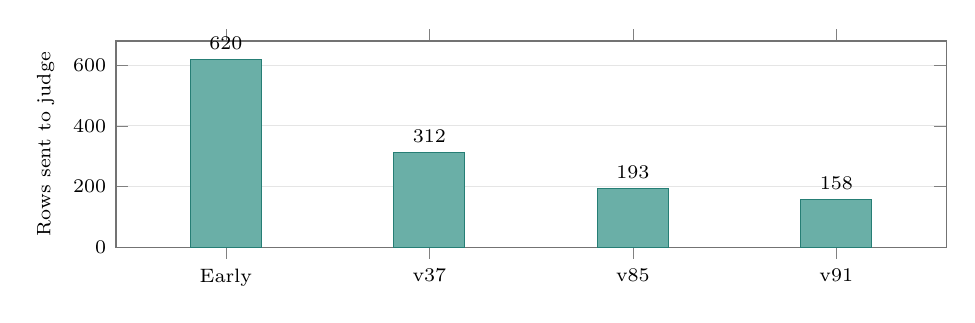
\begin{tikzpicture}
\begin{axis}[
  width=\columnwidth,
  height=42mm,
  ybar,
  bar width=9mm,
  ymin=0, ymax=680,
  ylabel={Rows sent to judge},
  symbolic x coords={Early,v37,v85,v91},
  xtick=data,
  nodes near coords,
  nodes near coords style={font=\scriptsize},
  tick label style={font=\scriptsize},
  label style={font=\scriptsize},
  axis line style={draw=black!55},
  ymajorgrids,
  grid style={black!10},
  enlarge x limits=0.18
]
\addplot[fill=huntrixteal!70, draw=huntrixteal!90!black]
coordinates {(Early,620) (v37,312) (v85,193) (v91,158)};
\end{axis}
\end{tikzpicture}
\caption{The deterministic router reduced the Phase 1 judge queue by 74.5\%.}
\label{fig:uncertain}
\end{figure}

\section{Experiments}

\subsection{Evaluation Protocol}

We used the 299 released labels for validation and error analysis, not as proof that a large fine-tune would transfer. We tracked macro-F1, F1 for each class, accuracy, and deterministic coverage. Context and no-context rows were inspected separately. Candidate rules were admitted only when they expressed a reusable relation and passed the regression suite.

The public leaderboard exposed roughly 30\% of Phase 1. A rounded score change therefore could not reveal a specific row label. We treated leaderboard results as aggregate evidence and retained the last reproducible anchor whenever a proposed correction regressed.

\begin{figure}[t]
\centering
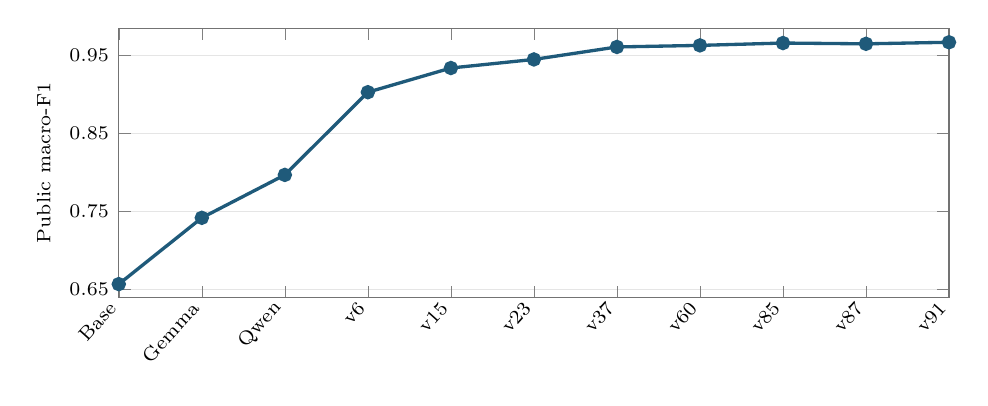
\begin{tikzpicture}
\begin{axis}[
  width=\columnwidth,
  height=50mm,
  xmin=0, xmax=10,
  ymin=0.64, ymax=0.985,
  xtick={0,1,2,3,4,5,6,7,8,9,10},
  xticklabels={Base,Gemma,Qwen,v6,v15,v23,v37,v60,v85,v87,v91},
  x tick label style={font=\scriptsize,rotate=48,anchor=east},
  ytick={0.65,0.75,0.85,0.95},
  tick label style={font=\scriptsize},
  label style={font=\scriptsize},
  ylabel={Public macro-F1},
  ymajorgrids,
  grid style={black!10},
  axis line style={draw=black!55}
]
\addplot[huntrixblue, very thick, mark=*, mark size=2pt]
coordinates {
 (0,0.657) (1,0.742) (2,0.797) (3,0.903) (4,0.934)
 (5,0.945) (6,0.961) (7,0.963) (8,0.966) (9,0.965) (10,0.967)
};
\end{axis}
\end{tikzpicture}
\caption{Public leaderboard progression. The largest gain followed the shift from uniform judging to source and task routing.}
\label{fig:score}
\end{figure}

\subsection{Scored Iterations}

Table~\ref{tab:versions} reports representative scored versions. The initial character and embedding models established a 0.657 to 0.663 floor. Gemma 12B QAT and the Qwen judge improved factual reasoning, but remained prompt-sensitive. v6 introduced source and structured routing and jumped to 0.903. Later gains came from lineage audits, stricter provenance, legal evidence, and relation guards rather than a larger model.

\begin{table}[t]
\caption{Representative leaderboard iterations}
\label{tab:versions}
\centering
\footnotesize
\begin{tabularx}{\columnwidth}{@{}l r X@{}}
\toprule
Version & Public F1 & Principal change \\
\midrule
Baseline & 0.657 & character and embedding models \\
Gemma & 0.742 & 12B QAT generic judge \\
Qwen & 0.797 & 27B lexical/factual judge \\
v6 & 0.903 & source and structured routing \\
v15 & 0.934 & expanded lineage, calibrated rules \\
v23 & 0.945 & provenance repair batch \\
v37 & 0.961 & source-lineage audit \\
v60 & 0.963 & conservative factual corrections \\
v85 & 0.966 & reproducible two-source anchor \\
v87 & 0.965 & plausible fact edits; reverted \\
v91 & \textbf{0.967} & typed idiom and relation guards \\
\bottomrule
\end{tabularx}
\end{table}

v91 changed five evidence-backed decisions from v85. Its public gain was 0.001, but the final private leaderboard score was 0.982, rank 1. This gap is consistent with the limited public split and is not presented as evidence that every v91 change generalized.

\subsection{Failed Approaches}

A prompt-vote ensemble obtained 0.8512 locally and 0.783 publicly. It overfit prompt behavior on the small released set. A compact TF-IDF verifier improved from 0.7879 to 0.8261 out of fold, but remained weak on no-context cultural facts. Raw external-QA retrieval often returned adjacent passages with the wrong relation or authority. A global context substring rule failed on instructional grammar contexts. Finally, v87 applied two externally plausible fact edits and fell from 0.966 to 0.965. We reverted it and tightened the admission policy.

After those runs, retrieval became a proposal mechanism, context rules became relation-aware, and each researched evidence record required a source and typed predicate. Candidate batches without a clear expected direction were quarantined instead of submitted.

\subsection{Released-Label Results}

\begin{table}[t]
\caption{Released-label evaluation}
\label{tab:local}
\centering
\footnotesize
\begin{tabular}{@{}lrr@{}}
\toprule
Metric & Full cascade & Deterministic subset \\
\midrule
Rows & 299 & 225 \\
Macro-F1 & 0.993264 & 1.000000 \\
F1, hallucinated (\labelzero) & 0.992701 & 1.000000 \\
F1, faithful (\labelone) & 0.993827 & 1.000000 \\
Accuracy & 0.993311 & 1.000000 \\
\bottomrule
\end{tabular}
\end{table}

The two remaining errors are internally inconsistent released controls. We left them unchanged rather than add row-specific exceptions.

\section{Reproducibility and Deployment}

The inference notebook reads the literal organizer path:

\begin{quote}
\code{/kaggle/input/competitions/}\\
\code{bengali-hallucination/test set.csv}
\end{quote}

It does not search for alternate filenames, branch on the row count, call an external API, or load a Phase 1 prediction vector. The organizers can replace the file mounted at that path for Phase 2 without editing a notebook variable.

\begin{table}[t]
\caption{Frozen deployment measurements}
\label{tab:runtime}
\centering
\footnotesize
\begin{tabularx}{\columnwidth}{@{}p{0.31\columnwidth}X@{}}
\toprule
Property & Frozen result \\
\midrule
Hardware & Kaggle Tesla T4$\times$2; internet disabled \\
Model & Qwen3.6-27B Q4\_K\_P, 16.332~GiB \\
Phase 1 runs & 440.87, 527.03, and 593.43 seconds \\
5,000 same-mix run & 876.14 seconds, or 14.60 minutes \\
Pessimistic bound & all rows, three views: about 5.2 to 5.5 hours \\
Output & 2,516 IDs; 1,181 zeros and 1,335 ones \\
SHA-256 & \code{0fec5d610f4e7b94...}\\
Tests & 249 repository tests passing at freeze \\
\bottomrule
\end{tabularx}
\end{table}

Three notebook runs produced byte-identical files matching competition submission 54836339. The full digest is published in the freeze manifest. The public package pins the notebook version, Qwen checkpoint, CUDA runtime, evidence dataset, hardware, and expected hash.

\subsection{Determinism Controls}

Reproduction depends on more than a fixed random seed. The notebook sorts unresolved IDs before scheduling work and uses fixed batch boundaries. It starts both \texttt{llama.cpp} servers with pinned command lines, waits for health checks, and assigns the same prompt view to the same server on every run. Generation is limited to one grammar-constrained token. The CSV writer preserves incoming IDs, writes integer labels, and uses a fixed column order. A final validation cell checks row count, sequential Phase 1 IDs when applicable, nulls, label values, counts, and SHA-256.

The SHA check is a Phase 1 reproduction check, not a Phase 2 condition. On the held-out file, the notebook validates schema and IDs but does not expect the Phase 1 digest or label distribution. This separation prevents the notebook from recognizing the Phase 1 file and switching to a stored result.

\subsection{Phase 2 Procedure}

The frozen notebook infers the row count and preserves incoming IDs. Before submission, we duplicated the current distribution to roughly 5,000 rows and verified schema, row-count independence, offline execution, and GPU memory. A same-mix run took 14.60 minutes. Because broader Phase 2 data may route fewer cases deterministically, we also estimated the case in which all 5,000 rows need all three LLM views. The resulting 5.2 to 5.5 hour bound remains below the nine-hour budget.

\subsection{Expected Domain Shift}

The organizer preview names Common Crawl, Bengali Wikipedia, Banglapedia, Bangladesh government pages, recent newspapers, legislation, NCTB textbooks, and Bengali literature sites \cite{phase2}. Phase 1 source lineage should therefore cover a smaller share of Phase 2. The system does not turn an unfamiliar source into an approximate lineage match. When exact source and relation checks fail, the row moves to context reasoning or the judge.

\begin{table}[t]
\caption{Phase 2 routing under the announced source mix}
\label{tab:shift}
\centering
\footnotesize
\begin{tabularx}{\columnwidth}{@{}>{\raggedright\arraybackslash}p{0.29\columnwidth}>{\raggedright\arraybackslash}X@{}}
\toprule
Source family & Primary handling and abstention condition \\
\midrule
Common Crawl and news & Context grounding; defer unsupported outside claims \\
Wikipedia and Banglapedia & Exact entity-relation match; no approximate override \\
Government services & Context clauses, dates, fees, offices, and named entities \\
Bangladesh laws & Exact act and section when present; otherwise judge \\
NCTB textbooks & MCQ, numeric, grammar, and context solvers \\
Literature sites & Exact work/author relation or reliability consensus \\
Unknown source & Skip lineage and use the fixed judge path \\
\bottomrule
\end{tabularx}
\end{table}

This fallback is deliberate. A loss of deterministic coverage increases runtime but is safer than forcing Phase 1 evidence onto new domains. The all-uncertain bound measures that failure mode directly. It also explains why the notebook keeps the 27B judge even though only 158 Phase 1 rows required it.

\subsection{Method and Rule Disclosure}

The router contains short citation-backed factual records researched from public sources for unlabeled prompts. It never used hidden labels, manually assigned row labels, paid APIs, or closed hosted inference. We told the organizers when exact prompt/source relationships were discovered and how the public-source records were built. They replied that Kaggle foundational rules were not organizer-imposed and that a solution without manually labeled rows, API calls, or other rulebook violations would not be disqualified. The pipeline still computes every output label from the provided row and its pinned evidence.

The public repository omits competition test data, predictions, credentials, and model weights. It includes the notebook, report, version manifest, citations, data-source register, third-party notices, form values, and run instructions. Model and runtime files remain on exact public Kaggle versions.

\begin{table}[t]
\caption{Published artifact boundary}
\label{tab:artifacts}
\centering
\footnotesize
\begin{tabularx}{\columnwidth}{@{}>{\raggedright\arraybackslash}p{0.28\columnwidth}>{\raggedright\arraybackslash}X@{}}
\toprule
Location & Contents \\
\midrule
GitHub & Notebook, LaTeX report, PDF, manifests, citations, and runbook \\
Kaggle Model & Pinned public Qwen3.6-27B quantization \\
Kaggle Dataset & Router evidence, \texttt{llama.cpp} CUDA build, notices \\
Competition mount & Organizer-provided CSV at the literal required path \\
Notebook output & Newly computed \texttt{submission.csv} only \\
Not published & Competition rows, scored predictions, credentials \\
\bottomrule
\end{tabularx}
\end{table}

\subsection{Limitations}

The private 0.982 result does not guarantee equal performance on broader Phase 2 sources. Exact lineage helps reproduce known source families but cannot replace general reasoning on new civic, legal, textbook, and news material. The 299 labels are too small to establish performance for every domain. Public-source records also require continuing license and provenance review. In a deployed civic system, unresolved legal or service information should be escalated rather than accepted from a binary detector alone.

\section{Conclusion}

Changing the unit of reasoning mattered more than enlarging the judge. Exact provenance and typed solvers handled cases with clear relations; a fixed open-weight model handled the remaining ambiguity. The result was more accurate than uniform LLM judging, fast enough for offline T4$\times$2 inference, and reproducible byte for byte from raw input. Each deterministic label identifies its evidence family, and every unresolved label follows a fixed prompt and voting path.

\begin{thebibliography}{00}

\bibitem{competition}
Sushmit, ``Bengali LLM Hallucination Detection Challenge,'' Kaggle, 2026. [Online]. Available:
\url{https://www.kaggle.com/competitions/bengali-hallucination}

\bibitem{phase2}
Competition organizers, ``Phase 2 Reveal + a Note on Data Resources,'' Kaggle Discussion, 2026.

\bibitem{benhallu}
``BenHalluEval: A Multi-Task Hallucination Evaluation Framework for Large Language Models on Bengali,'' 2026. [Online]. Available:
\url{https://arxiv.org/abs/2605.31483}

\bibitem{idiom}
``When Words Don't Mean What They Say: Figurative Understanding in Bengali Idioms,'' LREC 2026.

\bibitem{tydi}
J. H. Clark \emph{et al.}, ``TyDi QA: A Benchmark for Information-Seeking Question Answering in Typologically Diverse Languages,'' \emph{Transactions of the ACL}, vol. 8, pp. 454 to 470, 2020.

\bibitem{qwen}
Qwen Team, ``Qwen3.6-27B Q4\_K\_P,'' public Kaggle model, 2026.

\bibitem{llamacpp}
G. Gerganov \emph{et al.}, ``llama.cpp,'' GitHub repository, pinned build b9637, 2026. [Online]. Available:
\url{https://github.com/ggml-org/llama.cpp}

\end{thebibliography}

\end{document}
